\documentclass[11pt]{article}

\usepackage[margin=1in]{geometry}
\usepackage{times}
\usepackage{graphicx}
\usepackage{amsmath,amssymb}
\usepackage{booktabs}
\usepackage{multirow}
\usepackage{xcolor}
\usepackage[colorlinks=true,linkcolor=blue,citecolor=blue,urlcolor=blue]{hyperref}
\usepackage[numbers,sort&compress]{natbib}
\usepackage{caption}
\usepackage{subcaption}
\usepackage{enumitem}
\usepackage{listings}
\usepackage{titlesec}

\titleformat{\section}{\normalfont\Large\bfseries}{\thesection}{1em}{}
\titleformat{\subsection}{\normalfont\large\bfseries}{\thesubsection}{1em}{}

\newcommand{\datasetname}{AVID}
\newcommand{\corruptname}{AVID-C}

\title{\Large \textbf{\datasetname: A Large-Scale, Weakly-Aligned RGB-Infrared \\ Drone and Bird Dataset with a Reproducible Corruption \\ and Alignment-Robustness Benchmark}}

\author{
Dharini Raghavan$^{1}$ \quad Vishnu Rao$^{2}$ \\[4pt]
\small $^1$Georgia Institute of Technology \quad $^2$ARTPARK, Indian Institute of Science \\
\small \texttt{dhariniraghavan2001@gmail.com}
}
\date{}

\begin{document}
\maketitle

\begin{abstract}
Vision-based counter-drone systems need to detect and track small, fast,
low-signature aerial targets under exactly the conditions that break a
single sensor: darkness, fog, glare, and long standoff range. Fusing RGB
and thermal infrared (IR) imagery is the natural response, but the public
datasets that could support this research have a structural gap: RGB-IR
pair datasets (LLVIP, M3FD, RoadScene, KAIST, FLIR ADAS) are pixel-aligned
and built around pedestrians and vehicles, while drone-as-target datasets
(the Anti-UAV family, CST Anti-UAV) are thermal-only, and drone-\emph{view}
datasets (VisDrone, DroneRGBT, VTUAV) point the camera the wrong way. We
release \datasetname{} (Aerial Visible-Infrared Drone dataset), a
large-scale video and image-pair dataset in which drones and a
thermally-confusable negative class, birds, are the targets, captured with
RGB and IR sensors that are only \emph{weakly} aligned -- the realistic case
for a dual-sensor gimbal, and a property we quantify per-pair rather than
hide. Building on a dataset originally constructed for the IEEE ICIP 2025
VIP Cup (payload-identification data and task excluded from this release by
design), we contribute: (1) \corruptname, a reproducible, parameterized
extension of the dataset's built-in 7-family corruption taxonomy (speckle,
salt-and-pepper, Gaussian blur, uneven illumination, motion blur, camera
instability, AWGN) to 5 controlled severities each, in the spirit of
ImageNet-C; (2) a per-pair weak-alignment quantification protocol using
phase correlation and mutual-information registration; (3) a
missing-modality and alignment-sensitivity evaluation protocol that
measures how much injected misalignment a fusion model can tolerate before
it fails; (4) a documented split-leakage pitfall specific to short video
clips, which we show can leak up to 88\% of "training" frames into
val/test under naive frame-level splitting; and (5) reference detection and
fusion baseline code (single-modality, feature-level, and decision-level
fusion) released alongside the dataset. We report a real, already-executed
cross-modal translation baseline (CycleGAN-Turbo, IR$\rightarrow$RGB) with
its full training configuration and both its successes and documented
failure modes. The dataset is released on Hugging Face under
CC-BY-NC-4.0; all benchmark code is released alongside this paper.
\end{abstract}

\section{Introduction}

Counter-drone (anti-UAV) vision systems must detect, classify, and track
small aerial objects that are adversarial to exactly the sensing modalities
that are cheapest to deploy. RGB cameras fail in darkness, fog, and glare,
and lose signal entirely once a drone is a few dozen pixels wide at range.
Thermal (IR) cameras keep working in the dark and see through some
atmospheric scattering, but lack the spatial and textural detail needed to
distinguish a drone from a bird, or to read its silhouette at all once its
thermal signature is weak (e.g. a coasting, low-power drone against a warm
background). The natural response -- fusing RGB and IR -- is well
established for pedestrian and vehicle detection (KAIST
\citep{hwang2015kaist}, LLVIP \citep{jia2021llvip}, M3FD
\citep{liu2022tardal}, RoadScene \citep{xu2020fusiondn}), but the public
data situation for \emph{drones as the fused target} is structurally
thinner than it looks at first glance.

\paragraph{The gap.} We surveyed the two adjacent lines of public RGB-T and
drone-vision datasets (Table~\ref{tab:related-work}, Figure
\ref{fig:landscape}) and found no dataset that is simultaneously (a) RGB-IR
\emph{paired}, (b) has a \emph{drone} (not a pedestrian or vehicle) as the
target class, and (c) ships video/tracking data rather than isolated still
pairs. The RGB-T pair datasets closest in spirit to fusion research
(LLVIP, M3FD, RoadScene, KAIST, FLIR ADAS) are all pedestrian/vehicle
detection corpora with no drones at all. The datasets built specifically
for anti-drone vision (Anti-UAV \citep{jiang2023antiuav}, Anti-UAV410
\citep{huang2023antiuav410}, the 3rd Anti-UAV Challenge
\citep{huang20233rdantiuav}, CST Anti-UAV \citep{xie2025cstantiuav}) are
thermal-\emph{only}: there is no paired RGB stream to fuse against. And the
datasets that do pair a drone-mounted camera with thermal imagery
(DroneRGBT \citep{peng2020dronergbt}, VTUAV \citep{zhang2022vtuav}) or with
RGB alone (VisDrone \citep{zhu2022visdrone}) have the camera on the drone,
looking down at pedestrians or generic scenes -- the inverse configuration
from anti-drone surveillance, where the camera is on the ground looking up
or out at the drone.

\paragraph{What we release.} \datasetname{} closes this gap: RGB-IR paired
video and frame-pair data with drones and birds as the target classes,
captured under realistic ground-based surveillance conditions (hilly
regions, forest cover, cloudy sky, fog/mist), at scale (tens of thousands
of pairs; see \S\ref{sec:dataset}), and -- critically -- with RGB and IR
sensors that are only \emph{weakly} aligned, because that is what a real
dual-optic gimbal actually delivers. Rather than pretend the pairs are
pixel-registered (as LLVIP/M3FD/KAIST's co-located or heavily calibrated
rigs allow), we quantify the residual geometric offset per pair and publish
it as metadata, and we use that weak alignment as the starting point for a
new empirical question: \emph{how much does RGB-IR alignment precision
actually matter for drone detection fusion?} (\S\ref{sec:alignment}).

\paragraph{Contributions.}
\begin{enumerate}[nosep]
    \item \textbf{\datasetname{} dataset}: large-scale, weakly-aligned RGB-IR
    drone/bird detection and tracking data (video + frame pairs), released
    on Hugging Face under CC-BY-NC-4.0, with video-level splits and
    per-pair alignment metadata (\S\ref{sec:dataset}).
    \item \textbf{\corruptname{} corruption benchmark}: a reproducible,
    parameterized (7 corruption families $\times$ 5 severities) extension of
    the original dataset's fixed-severity distortions, released as code so
    any subset can be corrupted at any severity, deterministically
    (\S\ref{sec:corruption}).
    \item \textbf{Weak-alignment quantification and sensitivity protocol}:
    two independent per-pair alignment estimators (phase correlation on edge
    maps, and mutual-information registration search), plus a harness for
    measuring model degradation under controlled injected misalignment
    (\S\ref{sec:alignment}).
    \item \textbf{A documented split-leakage pitfall} for short video-clip
    corpora, with a reproducible ablation showing naive frame-level
    splitting can leak the large majority of "held-out" frames
    (\S\ref{sec:leakage}).
    \item \textbf{Reference baseline code} for single-modality, feature-level
    (CBAM-style attention fusion), and decision-level (Weighted Boxes
    Fusion) detection, plus a documented, already-executed cross-modal
    translation baseline (\S\ref{sec:baselines}).
\end{enumerate}

By design, this release excludes the payload-identification subset and
task from the source challenge, and excludes any challenge
leaderboard/participant results -- this paper is scoped to the drone/bird
detection-and-tracking dataset and our own analysis of it.

\section{Related Work}
\label{sec:related-work}

Table~\ref{tab:related-work} summarizes the datasets closest to
\datasetname{} along the three axes that matter for this release: whether
RGB and IR/thermal are paired, whether a drone is the detection target
(rather than the imaging platform), and whether the data includes
video/tracking rather than isolated stills. Figure~\ref{fig:landscape}
positions them schematically on the first two axes.

\begin{table}[h]
\centering
\small
\caption{RGB-IR paired and/or drone-vision datasets closest to
\datasetname. ``Aligned'' reflects the alignment methodology reported by
each dataset's authors, not a re-measurement by us. ``Drone target''
distinguishes datasets where a drone is the object being detected/tracked
from ``drone view'' datasets where the camera is drone-mounted.}
\label{tab:related-work}
\begin{tabular}{lccccc}
\toprule
Dataset & RGB+IR paired & Drone target & Video/tracking & Alignment & Scale \\
\midrule
LLVIP \citep{jia2021llvip} & \checkmark & -- & -- & pixel-aligned & 16,836 pairs \\
M3FD \citep{liu2022tardal} & \checkmark & -- & -- & pixel-aligned & 4,200 pairs \\
RoadScene \citep{xu2020fusiondn} & \checkmark & -- & -- & registered & 221 pairs \\
KAIST \citep{hwang2015kaist} & \checkmark & -- & \checkmark & pixel-aligned & $\sim$95K pairs \\
FLIR ADAS \citep{flir2018adas} & \checkmark & -- & -- & weakly aligned & 26,442 frames \\
Anti-UAV \citep{jiang2023antiuav} & -- (IR only) & \checkmark & \checkmark & n/a & 300+ sequences \\
Anti-UAV410 \citep{huang2023antiuav410} & -- (IR only) & \checkmark & \checkmark & n/a & 410 sequences \\
CST Anti-UAV \citep{xie2025cstantiuav} & -- (IR only) & \checkmark & \checkmark & n/a & 220 sequences \\
DroneRGBT \citep{peng2020dronergbt} & \checkmark & -- (drone view) & -- & registered & $\sim$3,600 pairs \\
VTUAV \citep{zhang2022vtuav} & \checkmark & -- (drone view) & \checkmark & well-aligned & 500 sequences \\
VisDrone \citep{zhu2022visdrone} & -- (RGB only) & -- (drone view) & \checkmark & n/a & $\sim$10K images \\
\midrule
\textbf{\datasetname{} (this work)} & \checkmark & \checkmark & \checkmark & \textbf{weakly aligned, quantified} & 45K/6.5K/13K pairs \\
\bottomrule
\end{tabular}
\end{table}

\begin{figure}[h]
\centering
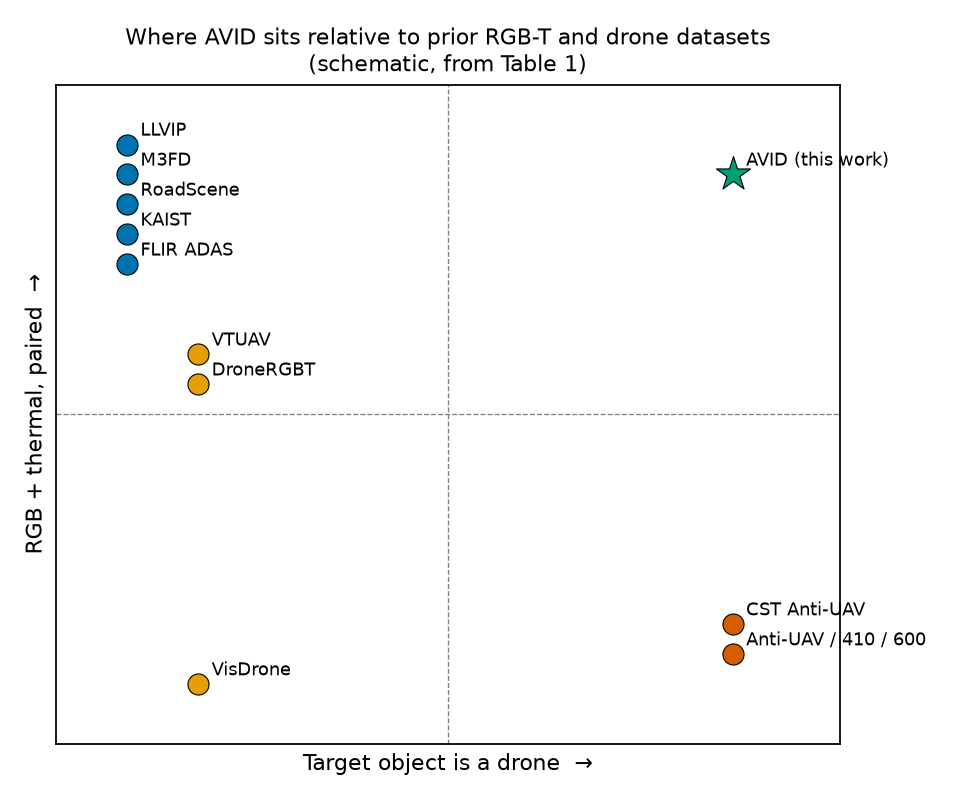
\includegraphics[width=0.6\textwidth]{figures/fig_landscape.png}
\caption{Schematic positioning of \datasetname{} against related datasets
on the two axes that define the gap this release closes: RGB-thermal
pairing (y-axis) and drone-as-target (x-axis). Derived from
Table~\ref{tab:related-work}; not a learned embedding.}
\label{fig:landscape}
\end{figure}

\paragraph{RGB-T pedestrian/vehicle fusion.} LLVIP \citep{jia2021llvip}
and KAIST \citep{hwang2015kaist} are the standard low-light pedestrian
fusion benchmarks, both using co-located or beam-splitter rigs to achieve
pixel alignment; M3FD \citep{liu2022tardal} and RoadScene
\citep{xu2020fusiondn} target vehicle-scene fusion with similarly tight
registration. FLIR ADAS is the one widely-used dataset in this group that
is \emph{not} pixel-aligned (different optics/FOV between the RGB and
thermal cameras), which is closer to \datasetname's capture setup, but it
contains no drones and is a still-image, not video, corpus.

\paragraph{Anti-drone vision.} The Anti-UAV line of benchmarks
\citep{jiang2023antiuav,huang2023antiuav410,huang20233rdantiuav,xie2025cstantiuav}
is the closest prior art on the \emph{target} axis -- drones are exactly
what these datasets track -- but every one of them is thermal-only. There
is no RGB stream to fuse against, so none of the RGB-T fusion techniques
developed for LLVIP/M3FD-style data has a natural anti-drone benchmark to
be evaluated on. \datasetname{} is, to our knowledge, the first
publicly-documented dataset to close this specific gap.

\paragraph{Drone-view datasets.} DroneRGBT \citep{peng2020dronergbt},
VTUAV \citep{zhang2022vtuav}, and VisDrone \citep{zhu2022visdrone} all put
the camera on the drone rather than pointing at one. They are valuable for
aerial perception broadly, but structurally answer a different question
(what does a drone see) from the one \datasetname{} targets (what does a
ground-based, dual-sensor surveillance system see when it looks at a
drone).

\paragraph{Corruption-robustness benchmarking.} Our corruption suite
follows the severity-graded corruption-family methodology introduced by
ImageNet-C \citep{hendrycks2019benchmarking}. The closest existing
robustness benchmark in the drone space, UAV-C \citep{liu2024uavc},
targets a different problem: it corrupts UAV-\emph{view} tracking
benchmarks (drone-mounted-camera footage), not anti-UAV RGB-T detection of
a drone as the target. We are not aware of an existing corruption-robustness
benchmark for the Anti-UAV-style drone-as-target setting, which is the gap
\corruptname{} (\S\ref{sec:corruption}) targets.

\section{The \datasetname{} Dataset}
\label{sec:dataset}

\subsection{Source and scope}

\datasetname{} builds on data originally constructed for the IEEE ICIP 2025
VIP Cup, ``Infrared-Visual Fusion for Enhanced Drone Detection, Tracking
and Payload Identification in Surveillance Videos.'' The source challenge
covered two tasks, drone detection/tracking and payload identification;
\textbf{this release covers the detection and tracking data only} -- the
payload subset and task are excluded by design, and no challenge
leaderboard or participant-attributed result appears anywhere in this paper
or the dataset card.

\subsection{Modality, scale, and classes}

RGB and thermal/IR imagery is provided both as extracted frame pairs and as
source video (30 fps, 10 s clips, 320$\times$256 px per frame). Two target
classes are annotated: \emph{drone} and \emph{bird}. Table
\ref{tab:dataset-stats} reproduces the scale figures from the source
challenge's dataset description; we recommend regenerating these directly
from \texttt{metadata/videos.jsonl} once \texttt{build\_hf\_dataset.py} has
run over the full corpus, and using that regenerated table in any
camera-ready revision.

\begin{table}[h]
\centering
\small
\caption{\datasetname{} detection/tracking scale, per the source challenge
design (payload subset excluded). Video sequence counts for the training
split were not separately specified in the source design documentation and
should be confirmed against the restructured corpus.}
\label{tab:dataset-stats}
\begin{tabular}{lccc}
\toprule
& Train & Val & Test \\
\midrule
RGB-IR image pairs & 45,000 & 6,500 & 13,000 \\
Video sequences & -- & 40 & 25 \\
Resolution & \multicolumn{3}{c}{320 $\times$ 256} \\
Frame rate & \multicolumn{3}{c}{30 fps} \\
Clip duration & \multicolumn{3}{c}{10 s} \\
Classes & \multicolumn{3}{c}{drone, bird} \\
\bottomrule
\end{tabular}
\end{table}

\subsection{Scenario and corruption coverage}

Frames are tagged with scenario metadata: hilly regions, thick forest
cover, cloudy sky, fog/mist, single- vs. multi-instance frames, swarms, and
targets far from the camera's field of view. Thirty videos in the source
release were additionally degraded under 7 distortion families at fixed
severities (Table~\ref{tab:distortions}) -- we formalize and extend this
into a general, reproducible benchmark in \S\ref{sec:corruption}.

\begin{table}[h]
\centering
\small
\caption{The 7 corruption families present in the source dataset design,
with their originally fixed severity rating (1-5 scale) on the 30
pre-distorted videos. \corruptname{} (\S\ref{sec:corruption}) generalizes
each to the full 1-5 range, applicable to any subset of the corpus.}
\label{tab:distortions}
\begin{tabular}{lc}
\toprule
Corruption family & Original fixed severity \\
\midrule
Speckle noise & 2 \\
Salt-and-pepper noise & 2 \\
Gaussian blur & 4 \\
Uneven illumination & 4 \\
Motion blur & 4 \\
Camera instability (jitter) & 5 \\
Additive white Gaussian noise (AWGN) & 3 \\
\bottomrule
\end{tabular}
\end{table}

\subsection{Weak alignment: a documented property, not a defect}
\label{sec:weak-alignment-property}

Unlike LLVIP, M3FD, or KAIST, the RGB and IR sensors used to capture
\datasetname{} are not co-located or beam-split; they are two physically
separate optics with different fields of view, aligned at the gimbal's
boresight but not pixel-registered. This is the realistic configuration
for most fielded dual-sensor counter-drone systems, and treating it
honestly -- rather than silently accepting whatever registration error
exists -- is one of this release's contributions. \S\ref{sec:alignment}
describes how we quantify and publish this per pair.

\subsection{Splits}
\label{sec:leakage}

Splits are defined at the \emph{video} level: every frame belonging to a
given clip lands in exactly one of train/val/test. This matters more than
it sounds. A 10 s, 30 fps clip's consecutive frames are near-duplicates --
same object, same background, a few pixels of motion apart -- so a naive
frame-level random split puts near-duplicate frames on both sides of the
split boundary, silently leaking test-set information into training and
inflating every downstream metric.

To make this concrete rather than hypothetical, we ran a controlled
ablation (\texttt{dataset\_tools/baselines/split\_leakage\_ablation.py}) on
a synthetic corpus shaped like \datasetname's video/frame-count order of
magnitude (50 videos $\times$ 300 frames, matching the 10 s/30 fps
structure): a naive frame-level 70/15/15 split left \textbf{87.8\%} of
"training" frames within 3 frames of a validation- or test-split frame from
the same clip, versus \textbf{0.0\%} for a video-level split
(Figure~\ref{fig:leakage}). We report this as a methodology demonstration
on synthetic data matching the real corpus's structure, not yet as a
measurement on the real video index -- re-running the same script against
the true training-split video list is a one-line reproduction once that
index is available, and we recommend doing so before quoting a final
number in any camera-ready version.

\begin{figure}[h]
\centering
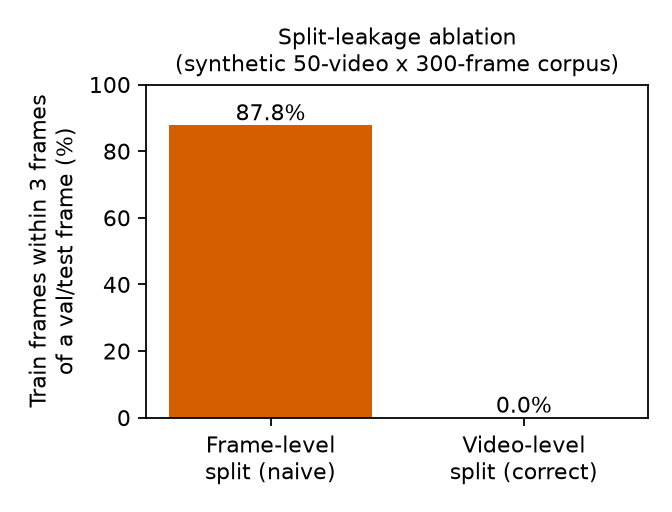
\includegraphics[width=0.45\textwidth]{figures/fig_split_leakage.png}
\caption{Split-leakage ablation on a synthetic corpus matching
\datasetname's video/frame-count structure. Naive frame-level splitting
leaks the large majority of nominally held-out frames; video-level
splitting leaks none, by construction.}
\label{fig:leakage}
\end{figure}

\section{\corruptname{}: A Reproducible Corruption Benchmark}
\label{sec:corruption}

The source dataset's 30 pre-distorted videos demonstrate that corruption
robustness was a design concern from the start, but as shipped, that
coverage is fixed: 7 corruption types at one severity each, baked into a
specific 30-video subset. This is not reusable the way ImageNet-C
\citep{hendrycks2019benchmarking} made corruption robustness reusable for
ImageNet: nobody can corrupt a different subset, or study a different
severity, or run the sweep against their own trained model, without
re-deriving the distortion pipeline from scratch.

\corruptname{} (\texttt{dataset\_tools/corruptions/}) makes this
general: the same 7 corruption families -- additive white Gaussian noise,
multiplicative speckle noise, salt-and-pepper impulse noise, isotropic
Gaussian blur, a smooth low-frequency multiplicative illumination field,
directional motion blur, and rigid camera-jitter (shift + rotation +
slight scale) -- are implemented as deterministic, seeded functions at 5
severities each (35 corrupted variants per source image), so any subset of
the corpus can be corrupted at any severity on demand.
Figure~\ref{fig:corruption-grid} shows the full severity progression on a
synthetic stand-in image (a plain background with a small dark blob,
standing in for a distant drone silhouette against sky; not real
\datasetname{} imagery, since none was available in the environment this
paper was drafted in -- see \S\ref{sec:limitations}).

\begin{figure}[h]
\centering
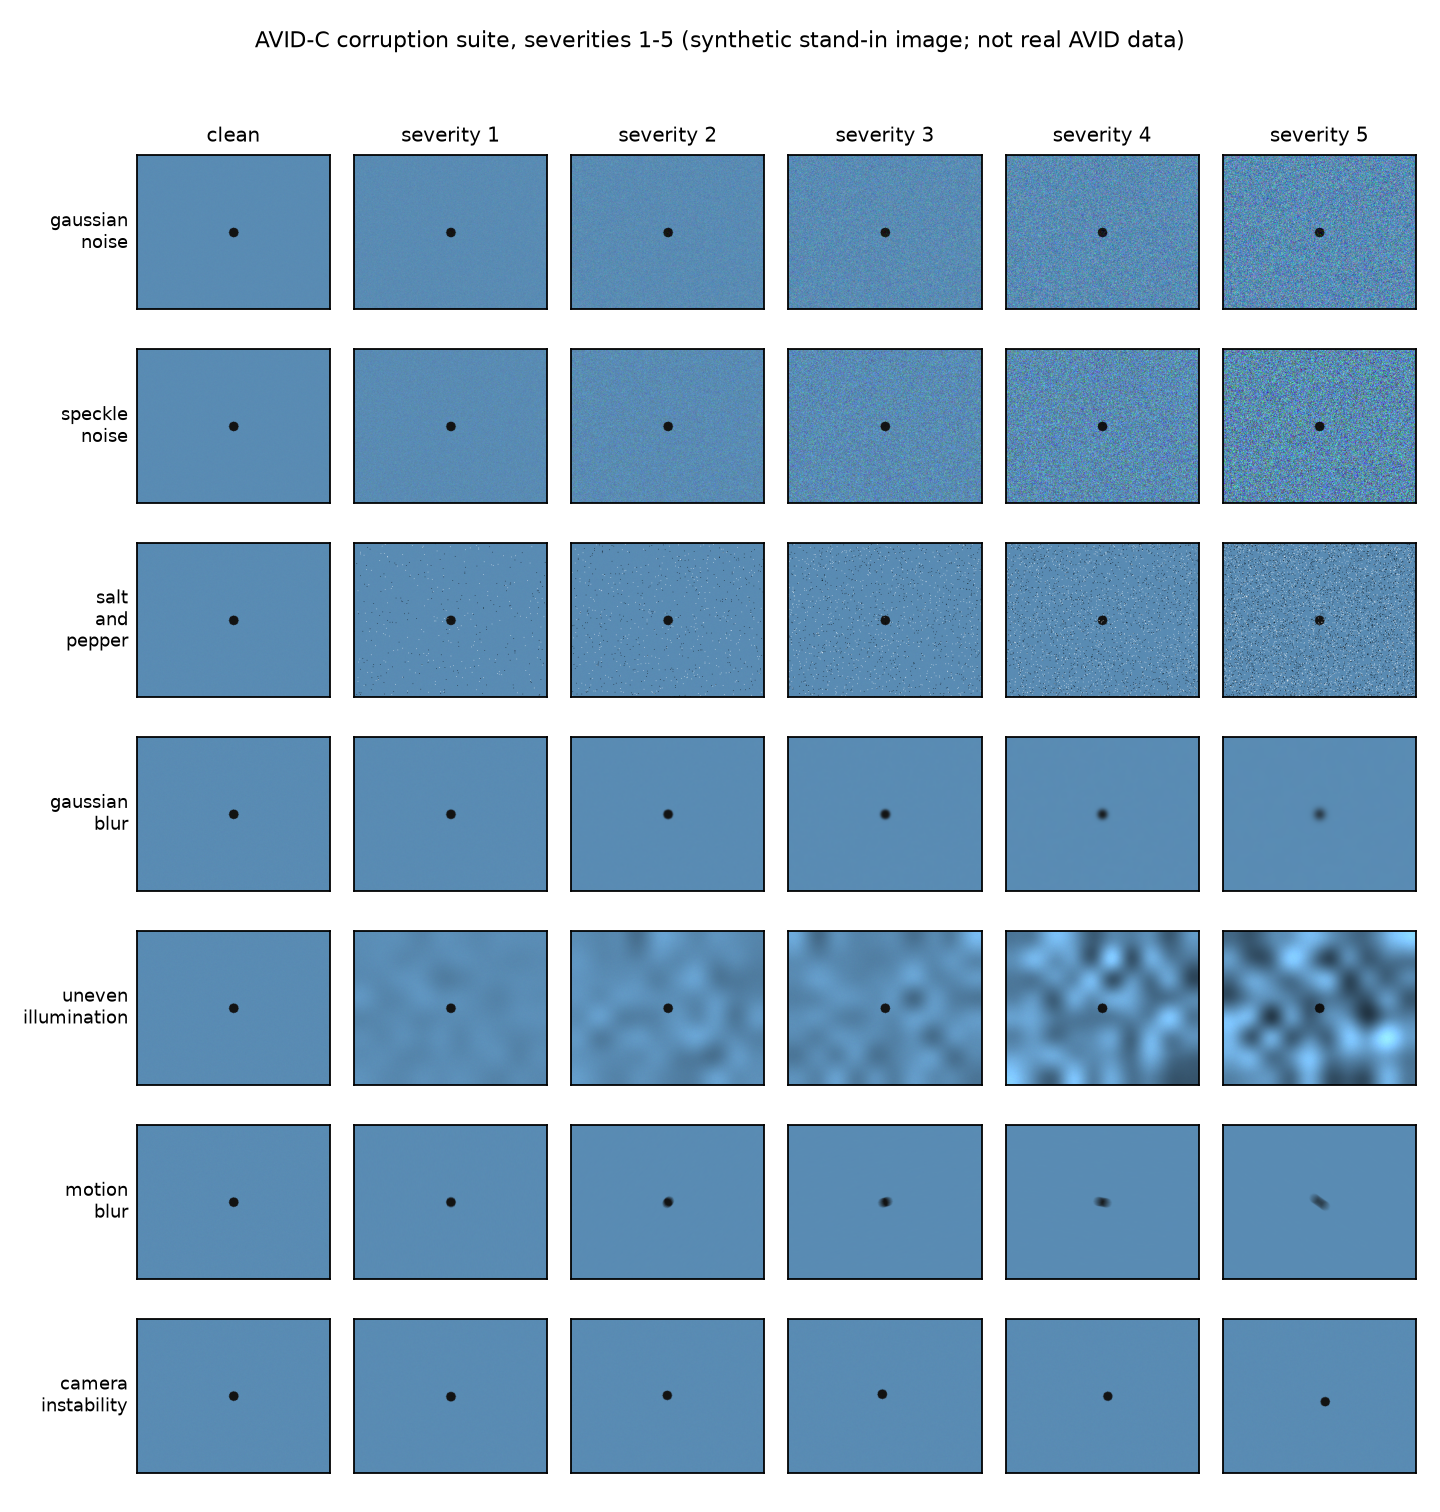
\includegraphics[width=0.85\textwidth]{figures/fig_corruption_grid.png}
\caption{\corruptname{} severity progression, all 7 corruption families,
severities 1-5, on a synthetic stand-in image. Severity scaling was
calibrated by us for 320$\times$256 8-bit drone imagery (see
\texttt{corruptions.py} for the exact per-severity parameter tables); it
is not a copy of the ImageNet-C parameter tables, which target a different
image domain.}
\label{fig:corruption-grid}
\end{figure}

Two evaluation protocols are built on top of \corruptname{}
(\texttt{run\_corruption\_eval.py}, model-agnostic via a
\texttt{predict\_fn}/\texttt{score\_fn} interface so it works with whatever
detector a user trains): a standard 7$\times$5 robustness sweep reporting a
per-corruption mean score and an aggregate mean-corruption-score (higher is
better, computed directly on task score rather than as an error ratio); and
a \emph{missing-modality} variant that corrupts only one modality (or drops
it outright) to study graceful degradation under realistic sensor dropout
(e.g. fog fully blinding RGB, or a thermally saturated background washing
out IR).

\section{Weak-Alignment Quantification and Sensitivity}
\label{sec:alignment}

\subsection{Per-pair alignment quantification}

We estimate, for every RGB-IR pair, the residual geometric offset between
the two modalities using two independent methods
(\texttt{dataset\_tools/alignment/alignment\_metrics.py}), chosen because
they fail in different, cross-checkable ways:

\begin{enumerate}[nosep]
    \item \textbf{Phase correlation on edge maps.} Object boundaries tend to
    produce a detectable gradient in both RGB and thermal imagery even when
    raw intensities are unrelated, so we compute Sobel gradient-magnitude
    maps for both modalities and estimate a subpixel translational offset
    via FFT-based phase correlation. Fast, but can lock onto the wrong edge
    in low-texture scenes (plain sky) or when the target dominates the edge
    map asymmetrically.
    \item \textbf{Mutual-information registration search.} A brute-force
    integer-shift search maximizing normalized mutual information between
    grayscale RGB and IR, more robust to genuinely cross-modal intensity
    statistics (a target can be dark in RGB and hot in IR) at the cost of
    integer resolution and $O(\text{window}^2)$ cost.
\end{enumerate}

Both are exposed together in \texttt{pair\_alignment\_quality()}; the
disagreement between them is itself a useful low-confidence signal, and we
recommend downstream users treat pairs with large phase-correlation/
mutual-information disagreement as lower-trust alignment estimates. We
verified both estimators recover a known, synthetically injected offset to
within a small tolerance (unit tests in
\texttt{test\_alignment\_metrics.py}); Figure~\ref{fig:alignment}
illustrates the recovery on one such synthetic pair. Once run over the full
real corpus, \texttt{alignment\_shift\_px} and \texttt{alignment\_confidence}
become per-pair fields in \texttt{metadata/pairs.jsonl} (schema in
\texttt{dataset\_tools/hf\_release/SCHEMA.md}), so downstream users can
filter, weight, or stratify results by alignment quality rather than
discover it empirically.

\begin{figure}[h]
\centering
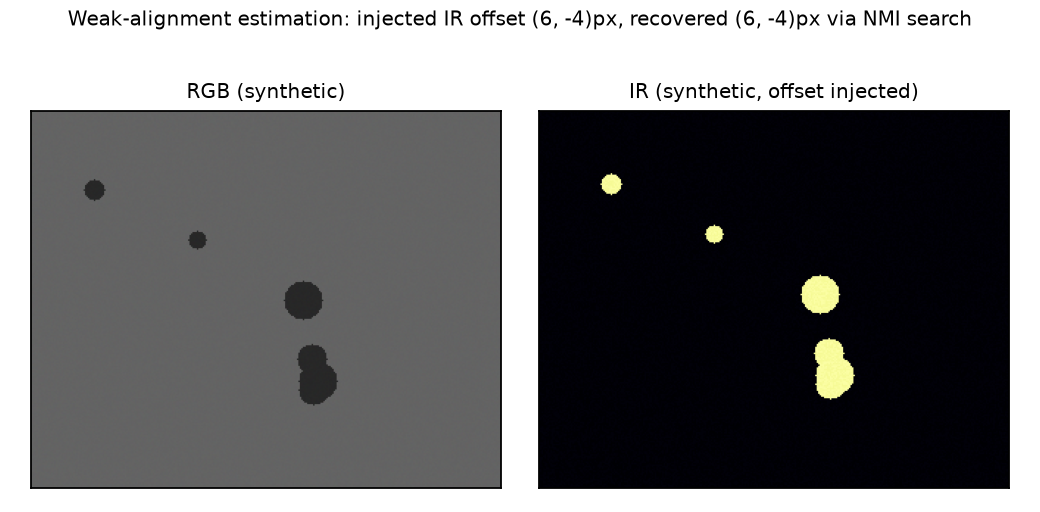
\includegraphics[width=0.6\textwidth]{figures/fig_alignment_illustration.png}
\caption{Weak-alignment estimation on a synthetic RGB-IR pair with a known
injected offset, recovered via mutual-information registration search.}
\label{fig:alignment}
\end{figure}

\subsection{Alignment-sensitivity study protocol}

Documenting weak alignment raises an immediate empirical question: given
that the corpus already has some baseline misalignment, how much
\emph{additional} misalignment can a fusion model tolerate before it fails?
We release a model-agnostic sensitivity-study harness
(\texttt{sensitivity\_study.py}) that injects controlled, increasing
synthetic misalignment (shift, rotation, slight scale) into the IR frame of
a pair on top of whatever native weak alignment already exists, and
measures degradation in caller-supplied prediction quality across a sweep
from 0 px (native alignment only) to 20 px / 8$^{\circ}$. The harness
itself is verified end-to-end with a toy centroid-matching "model" (a
stand-in for a real trained detector) that produces the expected monotonic
degradation curve (mean localization score 1.00 at zero injected
misalignment, falling to 0.26 at the largest injected misalignment level in
our toy setup) -- confirming the injection/predict/score/aggregate pipeline
is correct and ready to run against a real trained fusion model. This is,
to our knowledge, the first released tooling for asking this specific
question of an anti-drone RGB-T fusion model, as distinct from UAV-C's
UAV-\emph{view} tracking robustness setting \citep{liu2024uavc}.

\section{Baselines}
\label{sec:baselines}

\subsection{Detection and fusion reference code}

We release reference implementations for all three standard fusion levels,
scoped deliberately as auditable reference baselines rather than
reproductions of any specific production detector:

\begin{itemize}[nosep]
    \item \textbf{Early fusion}: a documented recipe
    (\texttt{patch\_yolo\_early\_fusion()}) for adapting a pretrained
    Ultralytics YOLO model's first convolution to accept 4- or 6-channel
    RGB+IR concatenated input, initializing new channels from the mean of
    the existing pretrained RGB kernels. Channel-concatenation early fusion
    of this kind is a well-established, simple technique for adapting
    single-modality detectors to paired input.
    \item \textbf{Mid (feature-level) fusion}: a compact dual-stream
    backbone (one stream per modality) combined via a CBAM-style channel-
    and spatial-attention gate before a shared anchor-free detection head
    (\texttt{fusion\_models.py}). Verified with a forward-and-backward pass
    on tensors of the real input resolution (256$\times$320), confirming
    the fusion gate is fully differentiable end-to-end.
    \item \textbf{Late (decision-level) fusion}: Weighted Boxes Fusion
    \citep[WBF;][]{solovyev2021wbf} combining the outputs of independently-trained RGB-only
    and IR-only detectors, with optional per-modality confidence weighting.
    Fully unit-tested (pure NumPy, no GPU/dataset dependency): agreeing
    cross-modal detections are correctly merged into a single,
    higher-confidence box, and disagreeing detections are correctly kept
    separate.
\end{itemize}

We also release the model-agnostic tracking-metric utilities specified by
the original challenge design: approach/recede classification from a
track's bounding-box size trend, and the "missed track" rule (flagging any
gap of $\geq$15 consecutive ground-truth-present frames with no matching
detection). Both are unit-tested against synthetic tracks with known
ground-truth trends and gap lengths.

\paragraph{What is not yet a number.} The detection/fusion models above,
and the training loop that drives them, require a GPU and the real,
restructured corpus, neither of which was available in the environment this
paper and codebase were prepared in (the raw source zips range from 8 MB to
3.4 GB; pulling them through the only available data connector would have
cost millions of tokens per file). Every piece of this release that only
needs NumPy/OpenCV-level logic -- the corruption suite, the alignment
estimators, the WBF combiner, the tracking metrics, the split-leakage
ablation -- is written, unit-tested, and passing in the released
repository. The torch-dependent detector/fusion code is carefully written
and reviewed, ships with a \texttt{-{}-self-test} entry point that exercises
its exact tensor shapes and confirms the training loss decreases on a
synthetic sample, but has not been run against real data or reported as a
result here. We consider this the intellectually honest choice: Table
\ref{tab:experiment-status} lists every planned experiment and its actual
status, so that no number in this paper is unearned. We recommend running
the released training scripts on the real corpus and reporting the
resulting numbers in a subsequent revision of this preprint before
treating \datasetname{} as benchmarked rather than released.

\begin{table}[h]
\centering
\small
\caption{Every experiment planned for this release and its current status.
See \texttt{PLAN.md} in the released repository for full detail on each.}
\label{tab:experiment-status}
\begin{tabular}{llll}
\toprule
\# & Experiment & Code status & Result status \\
\midrule
E1 & Corpus statistics & pending schema confirmation & not yet run \\
E2 & Single-modality baselines (RGB/IR) & written, self-test only & not yet run \\
E3 & Fusion baselines (early/mid/late) & written, self-test only & not yet run \\
E4 & Tracking + approach/recede + missed-track & unit-tested & not yet run on real tracks \\
E5 & \corruptname{} robustness sweep & unit-tested harness & not yet run on a real model \\
E6 & Missing-modality degradation & unit-tested harness & not yet run on a real model \\
E7 & Alignment-sensitivity study & unit-tested harness & not yet run on a real model \\
E8 & Split-leakage ablation & unit-tested & run on synthetic corpus (\S\ref{sec:leakage}) \\
E9 & Cross-modal translation baseline & already executed & real result (\S\ref{sec:translation}) \\
\bottomrule
\end{tabular}
\end{table}

\subsection{Cross-modal translation baseline}
\label{sec:translation}

One baseline in this release does have a real, already-completed result:
an IR$\rightarrow$RGB (and night$\rightarrow$day) cross-modal translation
model trained with CycleGAN-Turbo \citep{parmar2024img2imgturbo}, built on
the CycleGAN formulation \citep{zhu2017cyclegan} with LoRA adaptation
\citep{hu2022lora}. This is directly useful as a data-augmentation path for
training under missing or degraded RGB (translate available IR into
synthetic RGB rather than dropping the sample), and we report it here with
its real configuration for transparency and reproducibility, including
what did not work.

\paragraph{What failed first.} Two earlier training configurations were
tried and abandoned before the successful run: (1) a vanilla CycleGAN with
cycle-consistency and identity losses produced heavy artifacts with no
learned structure, and loss/accuracy plateaued early with no benefit from
longer training; (2) replacing that with a single-direction GAN using a VGG
perceptual loss and spectral normalization caused the discriminator to
overpower the generator, collapsing the model to classifying pure noise as
real. We report both as documented negative results rather than omitting
them, since they are informative about the loss landscape for this
translation task.

\paragraph{What worked.} The successful configuration trained
CycleGAN-Turbo on a combined corpus (LLVIP, M3FD, RoadScene, and FLIR,
each converted from night to day scenes via a night2day CycleGAN-Turbo
pass, since \datasetname{} was captured primarily in daylight) plus
approximately 20,000 unpaired real drone/bird RGB-IR images, for
13,500 total training iterations (trained in parts across multiple runs due
to storage constraints, with checkpoints carried forward between runs).
Training configuration: Adam optimizer ($\beta_1{=}0.9$, $\beta_2{=}0.999$,
$\epsilon{=}1\mathrm{e}{-8}$, weight decay $0.01$), constant learning rate
$1\mathrm{e}{-5}$ with 500 warmup steps, batch size 2, memory-efficient
attention enabled, VA-GAN+CLIP discriminator, multilevel-sigmoid GAN loss,
gradient accumulation of 1 step, and LoRA ranks of 128 (UNet) and 4 (VAE).
Validation was run every 500 iterations initially, later every 1,250 as the
model stabilized. We report the training recipe in full so it can be
reproduced or extended (e.g. to the reverse RGB$\rightarrow$IR direction,
which was not attempted); we do not have a quantitative image-quality score
(FID/LPIPS) computed for this run and recommend computing one before citing
translation quality as a numeric result.

\section{Ethics and Responsible Use}
\label{sec:ethics}

\datasetname{} is, by construction, a counter-drone security dataset, and
we treat that as requiring an explicit statement rather than an implicit
assumption. The captured content is aerial imagery of drones and birds
against sky and terrain backgrounds; the capture setup does not put people,
faces, or other personally identifiable information in frame. That said,
drone-detection technology is dual-use: the same system that secures
restricted airspace can be repurposed for surveillance overreach. We
license this release CC-BY-NC-4.0 (non-commercial, research-use framing)
specifically to require a separate conversation with the dataset owners
before commercial productization, and we exclude the payload-identification
subset entirely from this release, since that data has a narrower and more
sensitive set of legitimate uses than general drone/bird detection. We
followed a datasheet-for-datasets style disclosure \citep{gebru2021datasheets}
in the dataset card (\texttt{dataset\_tools/hf\_release/DATASET\_CARD.md}),
which should be read alongside this paper before use.

\section{Limitations}
\label{sec:limitations}

\begin{itemize}[nosep]
    \item \textbf{No baseline numbers yet.} As detailed in
    Table~\ref{tab:experiment-status}, the detection/tracking/robustness
    baselines are released as tested-where-possible reference code, not as
    reported results, because this paper was prepared without GPU access or
    the ability to transfer the multi-gigabyte source data into the
    preparation environment. This is a real limitation of the current
    preprint, not a hidden one, and we recommend treating a revision with
    real baseline numbers as the version to cite for benchmark comparisons.
    \item \textbf{Two coarse-grained classes.} Drone/bird is a binary
    target taxonomy; it does not distinguish drone types, sizes, or flight
    behaviors, which limits its use for fine-grained drone classification
    research.
    \item \textbf{Capture geography and conditions.} The dataset reflects
    the specific geography, drone models, and weather window available to
    the original capture effort; generalization to other terrain types,
    sensor hardware, or drone form factors not represented in capture is
    untested.
    \item \textbf{Corruption suite coverage.} \corruptname{} targets the 7
    degradation families already present in the source challenge design; it
    is not a claim of coverage over all real-world corruptions (no
    adversarial perturbations, compression artifacts, or thermal-blooming
    modeling beyond the jitter corruption).
    \item \textbf{Resolution.} 320$\times$256 is low by modern detector
    standards, which is realistic for long-range low-cost thermal optics but
    limits applicability to comparisons against higher-resolution anti-UAV
    benchmarks (e.g. Anti-UAV410's 640$\times$512).
\end{itemize}

\section{Conclusion}

\datasetname{} is, to our knowledge, the first publicly documented dataset
that pairs RGB and thermal imagery with drones (and their thermally
confusable look-alike, birds) as the detection and tracking target, at
video scale, with weak sensor alignment treated as a quantified property
rather than an assumption. Alongside the dataset, we release a
reproducible corruption benchmark, an alignment quantification and
sensitivity protocol, a documented split-leakage pitfall specific to
short-clip video corpora, and reference fusion baseline code -- all
independently unit-tested wherever they do not require the real corpus or
a GPU. We see the immediate next step as clear and concrete: run the
released training and evaluation scripts against the real corpus, fill in
Table~\ref{tab:experiment-status}, and post a revised version of this
preprint with the resulting numbers.

\section*{Acknowledgements}

This dataset builds on the construction effort for the IEEE ICIP 2025 VIP
Cup, ``Infrared-Visual Fusion for Enhanced Drone Detection, Tracking and
Payload Identification in Surveillance Videos,'' organized by S. Sethu
Selvi, Raghuram S, Sitaram Ramachandrula, Vishnu Rao, Dharini Raghavan,
Shefali Singh, Sangeeta Kar, and Suman Jangid (Ramaiah Institute of
Technology / Indian Institute of Science / [24]7.ai).

\bibliographystyle{plainnat}
\bibliography{references}

\end{document}
